\documentclass[letterpaper, 10 pt,onecolumn]{article}
\usepackage[english]{babel}
\usepackage[letterpaper,top=2cm,bottom=2cm,left=3cm,right=3cm,marginparwidth=1.75cm]{geometry}
% Useful packages
\usepackage{amsmath}
\usepackage{graphicx, float}
\usepackage[colorlinks=true, allcolors=blue]{hyperref}

\title{Lab 1 Report}
\author{Andre Winkel, Russell Yang}
\date{\today}

\begin{document}
\maketitle

\begin{abstract}
This lab will primarily focus on the use of QUARC and Simulink in order to interact with the hardware of the QUBE-Servo system, where QUARC is used to drive the DC motor and read the angular position of the disk. We will gain familiarity with the Quanser QUBE-Servo hardware, use QUARC to interact with the Quanser QUBE-Servo system, and acquire understanding of sensor calibration.
\end{abstract}

\section{System built}

\begin{figure} [H]
    \centering
    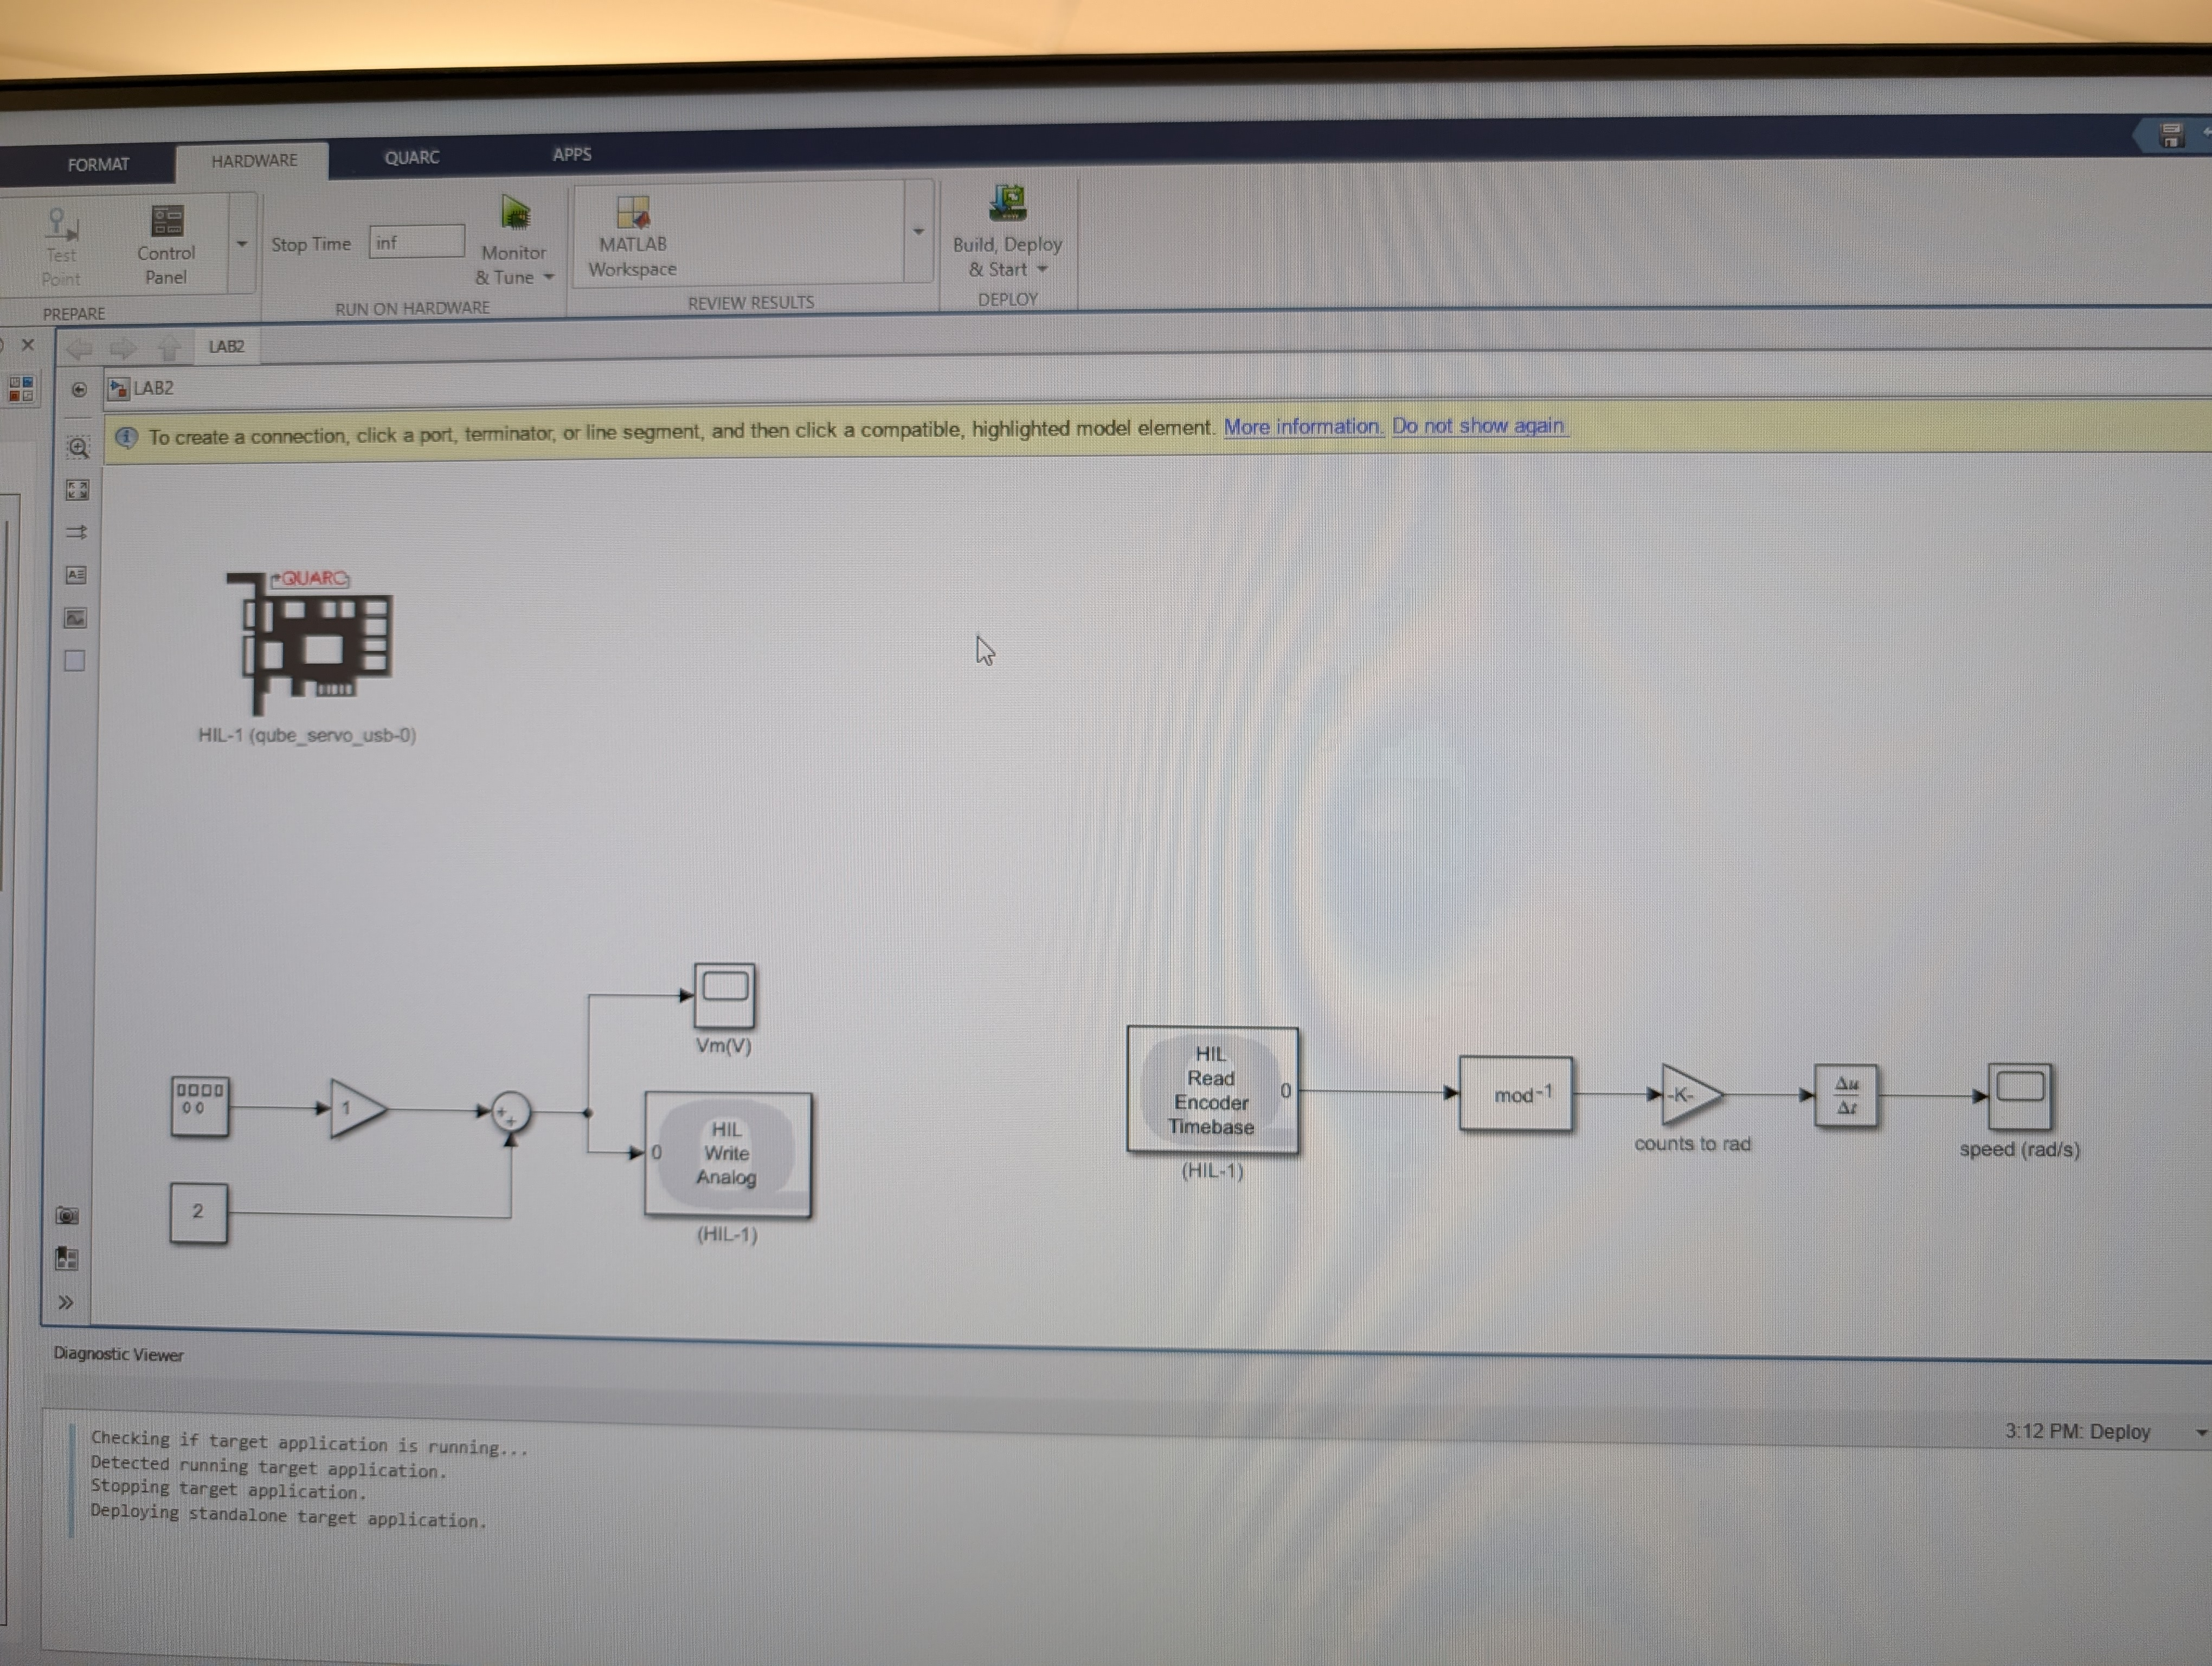
\includegraphics[width=0.4\linewidth]{1.jpg}
    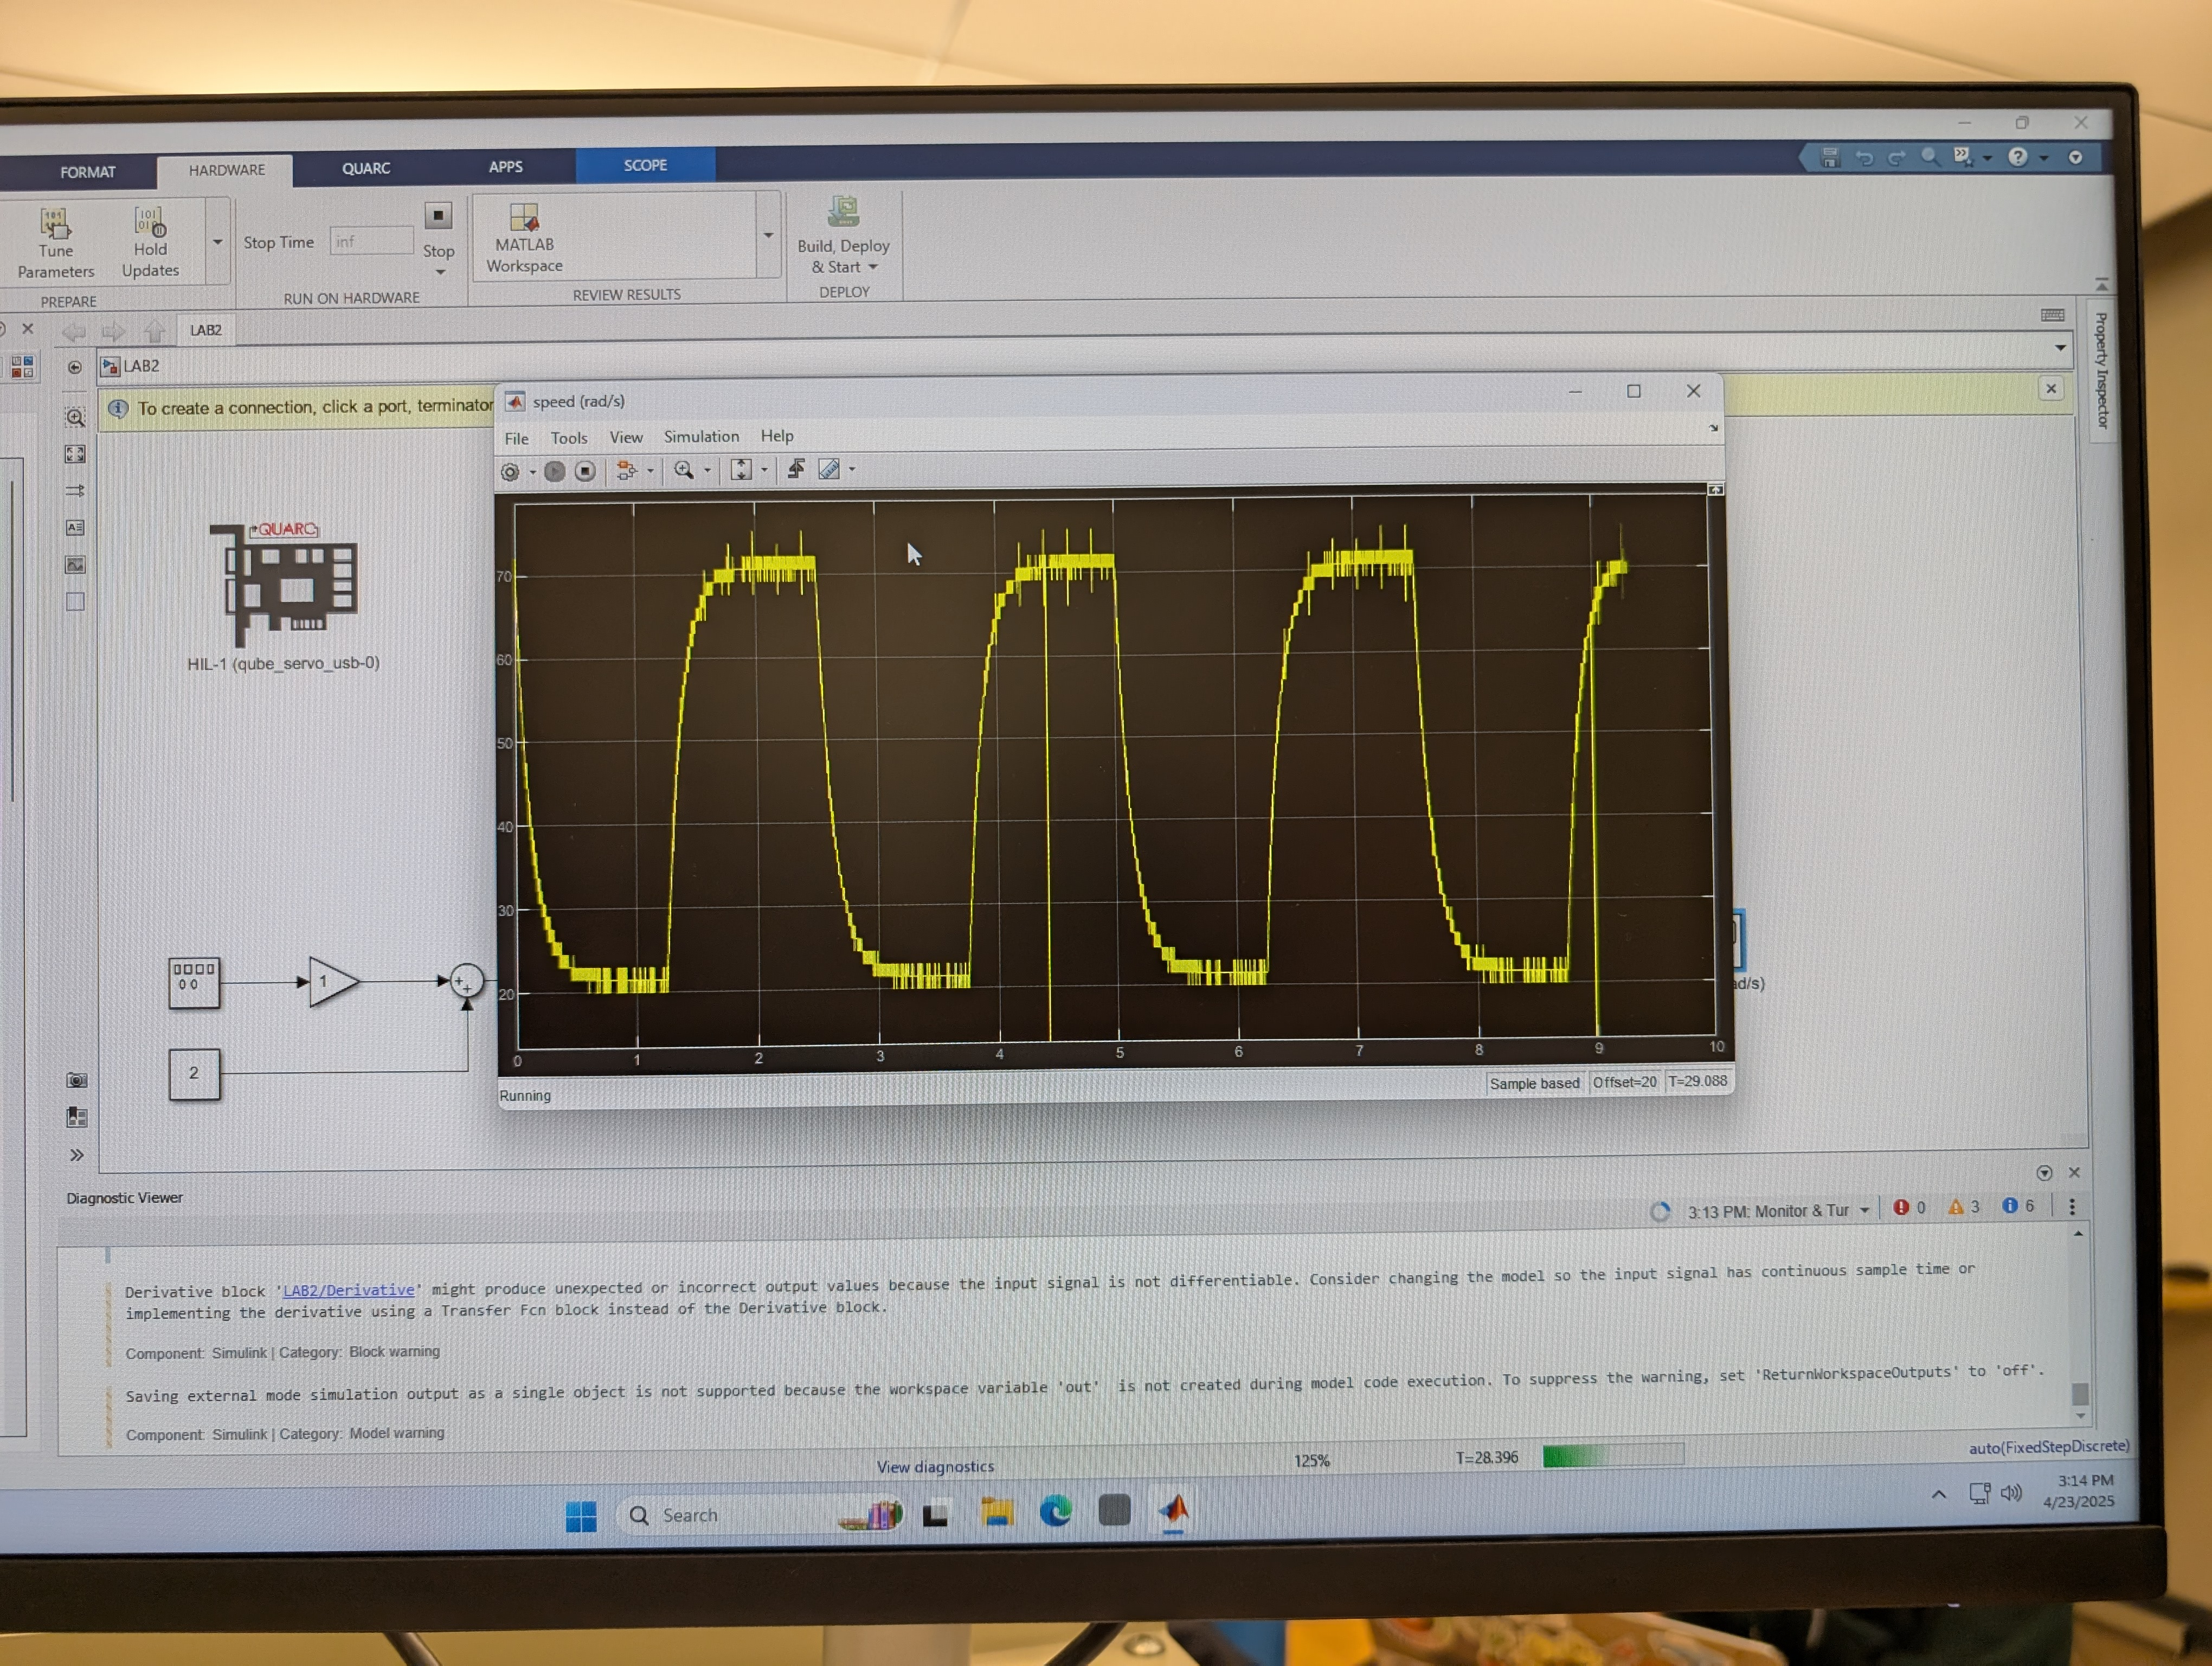
\includegraphics[width=0.4\linewidth]{2.jpg}
\end{figure}

\section{In-Lab Exercises and Results}
In this lab, we will use MATLAB and Simulink to build a model to read the angular position of the Quanser QUBE. 


\subsection{Reading the Encoder}
We used an encoder to read the counts which is proportional to the angle of the disk. We noticed that the encoder reading would reset to zero whenever we started the QUARC controller. When we stopped QUARC, rotated the disk and started QUARC again, we noticed that the physical position of the disk was now updated to be the zero location of the encoder count.
\subsection{Encoder Output for a Full Rotation}
For this measurement, we stopped the QUARC and lined up the line on the disk to the line on the QUBE. We then started the QUARC, effectively making that point the zero point. We then rotated the disk until the lines lined up once again. After 1 full rotation the encoder read 2048 counts. Therefore in order to set the gain to a value that converts the counts to degrees, we set the gain to $\frac{360}{2048}$. We repeated the above procedure and the display showed 360 degrees for a full rotation. 
\subsection{Driving the DC Motor}
For this section, we added an HIL Write Analog block and a Constant block to the Simulink diagram. We also added a Stall Monitor block to prevent damage to the motor. When we applied 0.5V to the DC motor by setting the constant block to 0.5, the disk rotated in counter-clockwise direction. Through this we can conclude that a positive input causes the motor to spin in the counter-clockwise direction and vice-versa for a negative input. 

\section{Analysis}
We effectively found how Simulink interacts with the QUBE. Primarily, it was understood that a full rotation of the motor gave an output of 2048, which we then used to manipulate to any number of our choice using a numerical constant. Additionally, we observed the reaction of the motor to a DC input of 0.5V through using a constant block, which resulted in a counter-clockwise spin. One of the main problems we faced was building and running our Simulink models \--- something we quickly figured out. Beyond this, our experiments were self-explanatory.

\section{Conclusion}
In this lab, we gained an understanding of Simulink and the QUBE Servo, and analyzed how they interact with each other. We additionally gained fundamental knowledge in building our Simulink models in order to collect data, as well as to transmit an output.

\end{document}